\chapter{Структуры событий для моделей памяти сохраняющих программный порядок}
\label{ch:porf-evenstruct}

В данной главе описан предложенный в диссертации метод 
кодирования слабых моделей памяти сохраняющих программный порядок 
с помощью простых структур событий с предикатом консистентности. 
Этот результат позволяет утверждать, что теория  
моделей памяти сохраняющих программный порядок%
\footnote{Везде далее в этом разделе 
под термином ``модель памяти'' будем подразумевать 
модель памяти сохраняющую программный порядок, 
если явно не утверждается иное.} 
может быть сведена к теории простых структур событий, 
и, как следствие, позволяет применить множество 
уже известных результатов о структурах событий%
~\cite{Winskel:86,Vaandrager:TCS1991,Sassone:MFCS1993,Nielsen:REX93,Winskel-TCS:09}
к проблемам слабых моделей памяти.

Теория простых структур событий и метод сведения 
моделей памяти к ним были формализованы в системе 
доказательства теорем \coq. 
Полученная в результате библиотека может быть использована 
для формализации доказательства свойств структур событий 
и моделей памяти, а также при разработке других
инструментов для интерактивной верификации многоточных программ.
%% Технические вопросы представления структур событий 
%% и других упоминаемых в данной главе формализмов 
%% также кратко рассматриваются в данной главе.  

Данная глава организована следующим образом. 
В разделе \cref{sec:pomset-graphs} описывается метод 
сведения графов сценариев исполнения к языкам помсетов. 
Далее, в разделе \cref{sec:mm-eventstruct} этот результат 
используется для сведения моделей памяти к простым структурам событий. 
В разделе \cref{sec:eventstruct-opsem} описывается 
операционная семантика для инкрементального построения 
структуры событий по заданной многопоточной программе 
и доказываются основные её свойства. 
%% Наконец, в \cref{sec:mm-eventstruct} кратко рассматриваются 
%% технические вопросы представления структур событий 
%% и других упоминаемых в данной главе формализмов.

\section{Сведение графов сценариев исполнения к языкам помсетов}
\label{sec:pomset-graphs}

%% Эквивалентность задания моделей памяти в терминах
%% графов сценариев исполнения и в терминах языков помсетов.

Напомним, что и формализм графов сценариев исполнения,
широко распространненый в сообществе для задания слабых моделей памяти%
~\cite{Alglave-al:TOPLAS14}, 
и формализм помсетов, известный по классическим работам%
~\cite{Pratt:CONCUR84,Gischer:TCS88} 
в области семантики многопоточных программ, основаны на теории частичных порядков. 
Главное отличие между ними заключается в том, что помсет состоит из единственного
отношения частичного порядка --- отношения причинно-следственной связи, 
в то время как граф сценариев исполнения состоит из
нескольких отношений, наделенных различной семантикой. 

Основная идея представленного метода сведения заключается в том 
что в рамках моделей сохраняющих программный порядок 
объединение отношения программного порядка и отношения ``читает-из''
может рассматриваться как аналог отношения причинно-следственной связи.
Таким образом множество графов сценариев исполнения можно факторизовать 
по отношению эквивалентности индуцированных отношений причинно-следственной связи.
И наоборот, можно построить частичную функцию, 
которая принимая на вход помсет и пытается выполнить 
разбиение отношение причинно-следственной связи на 
программный порядок и отношение ``читает-из''. 

Рассмотрим данное построение более формально. 
Для начала, введем формальное определение 
аксиоматических моделей памяти сохраняющих программный порядок.

\begin{definition}
Будем говорить, что граф сценария исполнения $G$ 
сохраняет программный порядок, если выполняются следующие условия: 
\begin{itemize}
  \item $G.\lR \suq \cod{G.\lRF}$; 
    \labelAxiom{$\lRF$-complete}{ax:rf-complete}

  \item $\lPO \cup \lRF$ является ацикличным отношением.
    \labelAxiom{$\lPORF$-acyclic}{ax:porf-acyc}
\end{itemize}
Обозначим множество всех таких графов как $\PorfExecG$.
Также будем говорить, что модель памяти $M$, 
заданная в аксиоматическом стиле, сохраняет программный порядок, 
если для любой программы $P$ каждый соответствующий ей
граф сценария исполнения $G \in \sem{P}_M$ сохраняет программный порядок, 
то есть ${\sem{P}_M \suq \PorfExecG}$.
\end{definition}

Далее определим функцию для построения помсета по графу сценария исполнения.

\begin{definition}
Определим функцию $\gpom : \PorfExecG \fun \Pom[\TidMemLab]$ следующим образом. 
Пусть $G \in \PorfExecG$. Тогда $\gpom(G) = \tup{E, \lab, \ca}$ где
\begin{itemize}
  \item $E = G.\lE$, 
  \item $\lab(e) = \tup{G.\lTID(e), G.\lLAB(e)}$,
  \item $\ca {}\defeq{} (G.\lPO \cup G.\lRF)^*$.
\end{itemize}
\end{definition}

Также предъявим обратную функцию, выполняющую построение 
графа сценария исполнения по помсету.
Для этого сначала определим подмножество помсетов, 
для которых такое построение возможно. 

\begin{definition}
Пусть $p = \tup{E, \lab, \ca} \in \Pom[\TidMemLab]$
и пусть $\simeq$ это некоторое отношение эквивалентности на метках событий. 
Будем называть помсет $p$ \emph{разделяемым на потоки относительно $\simeq$} 
(\emph{threaded pomset}) если для любого класса эквивалентности $\eset \suq E$
относительно $\simeq$ верно, что сужение помсета на события этого класса $p\rst{\eset}$ 
порождает линейно упорядоченное мультимножество. 
Множество всех таких помсетов будем обозначать как $\ThrdPom[\TidMemLab, \simeq]$.
\end{definition}

\begin{definition}
Пусть $p = \tup{E, \lab, \ca} \in \ThrdPom[\TidMemLab, \lEQTID]$. 
В таком случае определим индуцированное отношение 
программный порядка следующим образом:
$$ \lPO(p) \defeq \sca \cap \lEQTID. $$
Также определим множество кандидатов 
на отношение ``читает-из'' $\lRFs(p)$ 
таким образом, что $\lRF \in \lRFs(p)$ 
при выполнении следующих условий:
\begin{itemize}
  \item $\lRF {}\suq{} \lEQLOC \cap \lEQVAL$,
  \item $E \cap \lR \suq \cod{\lRF}$, 
  \item $\ca {}={} (\lPO(p) \cup \lRF)^*$.
\end{itemize}
%
Соответствующим образом определим 
множество графов-кандидатов $\ExecGs{p}$. 
Положим $G \in \ExecGs{p}$ если $p \in \ThrdPom[\TidMemLab]$
и выполнены следующие условия:
\begin{itemize}
  \item $G.\lE = E$,
  \item $\tup{G.\lTID(e), G.\lLAB(e)} = \lab(e)$, 
  \item $G.\lPO = \lPO(p)$, 
  \item $G.\lRF \in \lRFs(p)$. 
\end{itemize}
Если же $p \not\in \ThrdPom[\TidMemLab]$ то положим $\ExecGs{p} = \emptyset$.
%
Понятие множество графов-кандидатов также можно расширить на уровень языков помсетов:
$$ \ExecGs{P} \defeq \set{ G ~|~ \exists p \in P \ldotp G \in \ExecGs{p} }. $$
%
Множество всех помсетов для которых $\ExecGs{p} \neq \emptyset$
будем обозначать как $\PorfPom[\TidMemLab]$.
Также зададим частично определенную функцию 
${\pomg : \Pom[\TidMemLab] \pfun \ExecG}$,
которая для данного помсета выбирает 
один из соответствующих ему графов.
\begin{equation*}
  \pomg(p) = \begin{cases*}
    G      & такой что $G \in \ExecGs{p}$   \\
    \bot   & если $\ExecGs{p} = \emptyset$. \\
  \end{cases*}
\end{equation*}
%
\end{definition}

\begin{proposition}
Для любого помсета $p \in \Pom[\TidMemLab]$
верно, что $\ExecGs{p} \suq \PorfExecG$
и, следовательно, $\pomg(p) \in \PorfExecG$.
\end{proposition}

Наконец, покажем, что произвольная модель памяти
сохраняющая программный порядок может быть 
представлена как язык помсетов. 

\begin{definition}
Пусть $M$ --- это заданная в аксиоматическом стиле 
модель памяти сохраняющая программный порядок,
то есть $M \suq \PorfExecG$.
Построим соответствующий ей язык помсетов 
$\wmmlang{M} \in \Pomlang[\TidMemLab]$ следующим образом.
Будем считать, что помсет принадлежит этому языку, 
если найдется хотя бы один граф, допустимый $M$,
который соответствует этому помсету: 
$$ p \in \wmmlang{M} \defeq \exists G \in \ExecGs{p} \ldotp G \in M. $$
\end{definition}
 
\section{Кодирование модели памяти с помощью структуры событий}
\label{sec:mm-eventstruct}

В предыдущем разделе было показано, что 
модель памяти сохраняющая программный порядок 
может быть представлена как язык помсетов. 
Это наблюдение позволяет заключить, 
что модель памяти также может быть представлена 
и как простая структура событий с предикатом консистентности,
ведь, как было упомянуто в разделе~\cref{sec:pomsets-eventstruct}, 
данный класс структур событий позволяет выразить произвольный язык помсетов. 

В этом разделе будет также показано,
что на самом деле модель памяти сохраняющая программный порядок 
может быть представлена как простая структура событий специального вида.
В данной структуре событий все события одного потока образуют дерево. 
Ветви этого дерева соответствуют различным путям исполнения данного потока,
а события, принадлежащие разным веткам дерева, находятся в отношении конфликта. 
Cтруктуры событий данного вида будем называть 
\emph{разделяемыми на потоки} (\emph{threaded prime event structures}).

Основной особенностью структуры событий принадлежашей 
данному подклассу является то,
что она может быть закодирована с помощью 
только одного отношения частичного порядка
и некоторого отношения эквивалентности на метках.
Отношение конфликта при этом не требуется хранить явно, 
оно индуцируется двумя предыдущими отношениями. 
Такое представление, зачастую, позволяет существенно 
упростить рассуждения о структурах событий. 
Например, можно заметить, что две структуры событий 
данного класса изоморфны тогда и только тогда, 
когда они изоморфны как помеченные частично упорядоченные множества. 

Введем формальные определения описанных выше объектов. 

\begin{definition}
Частично упорядоченное множество $\tup{E, \ca}$ 
называется \emph{префиксно-линейно упорядоченным} 
(\emph{downward-total}) если выполняется следующие условие:
$$ x \ca z \wedge y \ca z \implies x \ca y \vee y \ca x. $$
Если в дополнение к этому частично упорядоченное множество являетя 
префикс-конечным, то будем называть такое множество \emph{лесом}.
Если кроме того существует наименьший элемент $e_0 \in E$, 
тогда будем называть такое множество \emph{деревом}, 
а $e_0$ --- корнем этого дерева. 
\end{definition}

\begin{proposition}
Для леса $\tup{E, \ca}$ можно задать 
частично определенную функцию $\pred : E \pfun E$, 
возращающую родителя данного элемента: 
$$ \pred(e) = e' \;{}\iff{}\; e' \ica e $$
\end{proposition}

\begin{proposition}
Размеченный лес $\tup{E, \lab, \ca}$ порождает простую структуру событий 
без волнений (confusion-free) $S(p) = \tup{E, \lab, \ca, \cf}$, 
где отношение непосредственного конфликта задается следующим образом: 
$$ e_1 \icf e_2 \defeq e_1 \neq e_2 \wedge \pred(e_1) = \pred(e_2). $$
Далее в этом разделе для обозначения структуры событий, порождаемой $p$, 
будем писать просто $S$, если $p$ можно вывести из контекста. 
\end{proposition}

\begin{definition}
Пусть $S = \tup{E, \lab, \ca, \cf} \in \PrimeES[L]$ --- 
это простая структура событий
с бинарным конфликтом, и пусть $\simeq$ это некоторое 
отношение эквивалентности на метках $L$.
Рассмотрим сужение структуры событий на классы эквивалентности 
${ S\rst{\simeq} \defeq \tup{E, \lab, \ca {}\cap{} \simeq, \cf {}\cap{} \simeq} }$.
Будем говорить, что структура \emph{разделима на потоки относительно отношения $\simeq$}
если $S\rst{\simeq}$ образует размеченный лес и, кроме того, 
отношение конфликта во всей структуре событий является 
продолжением отношения конфликта в суженной структуре, то есть 
$${ \icf_S = \icf_{S\rst{\simeq}} }.$$
Будем обозначать множество всех таких структур 
как $\ThrdPrimeES[L,\simeq]$
\end{definition}

\begin{proposition}
Пусть $p = \tup{E, \lab, \ca}$ это 
размеченное частично упорядоченное множество, 
а $\simeq$ отношение эквивалентности на метках событий.
Предположим, что сужение отношения порядка на классы эквивалентности 
${ p\rst{\simeq} \defeq \tup{E, \lab, \ca {}\cap{} \simeq} }$ образует лес.
Рассмотрим отношение непосредственного конфликта $\icf$, порождаемое этим лесом. 
Если отношение $\cf$, определенное как продолжение $\icf$ вдоль отношения $\ca$,
иррефлексивно, тогда $\tup{E, \lab, \ca, \cf}$ является 
простой структурой событий разделимой на потоки относительно отношения $\simeq$.  
\end{proposition}

Рассмотрим структуру событий $S \in \ThrdPrimeES[\TidMemLab, \lEQTID]$
разделяемую на потоки относительно отношения $\lEQTID$.
Определим множество графов, которые она кодирует, следующим образом:
$$ \ExecGs{S} \defeq \ExecGs{\pomlang{S}}  $$

Для данной модели памяти $M$ можно дополнить $S$ предикатом консистентности, 
который будет отфильтровывать все конфигурации, 
не принадлежащие языку $\wmmlang{M}$.

\begin{definition}
Пусть ${S = \tup{E, \lab, \ca, \cf} \in \ThrdPrimeES[\TidMemLab, \lEQTID]}$
и ${M \suq \PorfExecG}$.
Определим простую структуру событий с предикатом консистентности
${\wmmpes{S}{M} = \tup{E, \lab, \ca, \cons}}$ таким образом, что:
\begin{itemize}
  \item $E {}\defeq{} E_S$,
  \item $\lab {}\defeq{} \lab_S$,
  \item $\ca {}\defeq{} \ca_S$,
  \item $C \in \cons {}\defeq{} C \not\in \gcf_S \wedge S\rst{C} \in \wmmlang{M}$.
\end{itemize}
\end{definition}

Корректность структуры событий $\wmmpes{S}{M}$ относительно языка 
порождаемого $M$ вытекает напрямую из определения. 

\begin{proposition}
\label{prop:thrd-es-sound}
Для любой структуры событий $S = \ThrdPrimeES[\TidMemLab, \lEQTID]$
и любой модели памяти $M \suq \PorfExecG$
язык помсетов, порождаемый $\wmmpes{S}{M}$, 
корректен относительно языка $\wmmlang{M}$, то есть:
$$ \pomlang{\wmmpes{S}{M}} \suq \wmmlang{M}. $$
Из этого, в частности, следует что:
$$ \ExecGs{S} \suq M. $$
\end{proposition}

Тем не менее, нетрудно заметить, что структура событий $\wmmpes{S}{M}$
не обязана быть полной относительно языка порождаемого $M$.
В следующем разделе будет рассмотрена операционная семантика 
для инкрементального построения структуры $S$ 
порождающей структуру $\wmmpes{S}{M}$ 
полную относительно языка $\sem{P}_M$ для 
любой заверщающейся программы $P$.

\section{Операционная семантика построения структуры событий}
\label{sec:eventstruct-opsem}

В данном разделе представлена операционная семантика 
для инкрементального построения структуры событий.
Предложенная семантика предоставляет конкретную
процедуру построения структуры событий, 
кодирующую все возможные сценарии поведения 
заданной программы~$P$ в заданной модели памяти~$M$.  
Также доказываются основные свойства данной семантики, 
а именно \emph{конфлюэнтность}, \emph{полнота} и \emph{терминируемость}.

Отметим, что помимо модели памяти $M$, данная семантика также параметризована
последовательной семантикой потоков программы $P$, 
заданной в терминах системы помеченных переходов $\LTS$. 
Это, в частности, позволяет абстрагироваться от деталей 
реализации последовательной семантики 
и комбинировать предложенную семантику построения структуры событий 
с различными моделями последовательных вычислений. 

Прежде чем перейти к рассмотрению операционной семантики, 
введем несколько вспомогательных определений, 
помогающих связать структуру событий с 
последовательной семантикой. 

\begin{definition}
Пусть $\LTS = \tup{\State, L, \ltr{}{}{}}$ это система помеченных переходов, 
а $p = \tup{E, \lab, \ca}$ это лес размеченный метками типа $\Step{L}{\State}$. 
Будем говорить, что $p$ \emph{корректен} (\emph{sound}) 
относительно $\LTS$ если выполняются следующие условия:
\begin{itemize}
  \item для любого события $e \in E$ его метка 
    $\lab(e) = \step{l}{\state}{\state'}$ 
    образует валидный переход, то есть $\ltr{l}{\state}{\state'}$;
  %
  \item метки соседних событий $e_1 \ica e_2$ \emph{сопряжены} в том смысле, что если 
    $\lab(e_1) = \step{l_1}{\state_1}{\state'_1}$ и 
    $\lab(e_2) = \step{l_2}{\state_2}{\state'_2}$ тогда 
    $\state'_1 = \state_2$.
\end{itemize}
Будем говорить, что структура событий разделимая на потоки
корректна относительно системы переходов, 
если соответствующей этой структуре лес корректен. 
\end{definition}

\begin{proposition}
Пусть $p$ это лес, корректный относительно системы переходов~$\LTS$.
Тогда для любого событий $e \in E$ верно, что
метки событий его префикс $\dwset{e}$, упорядоченного согласно отношению $\ca$, 
образуют валидную трассу системы $\LTS$.

Аналогичное утверждение верно для структуры событий разделимой на потоки,
с точностью до того, что для такой структуры необходимо сузить
префикс на события того же потока, что и рассматриваемое событие $e$.  
\end{proposition}

Для того чтобы хранить локальные состояния потоков в структуре событий
дополним тип меток $\TidMemLab$ до типа 
$\ThrdMemLab \defeq \Tid \times \Lab \times \State \times \State$
расширив его парой состояний, формирующих переход.
Также определим функцию $\lSTEP$, извлекающую из метки $\ell \in \ThrdMemLab$ 
тройку образующую помеченный переход:
$$ \lSTEP(\tup{t, \el, \state, \state'}) = \step{\el}{\state}{\state'}. $$

Для удобства при необходимости мы также будем трактовать 
структуру событий $S \in \PrimeES[\ThrdMemLab]$ как 
структуру с метками типа $\TidMemLab$, то есть 
$S \in \PrimeES[\ThrdMemLab]$.

\begin{definition}
Предположим, что многопоточная программа $P$ задана как 
система помеченных переходов $\LTS = \tup{\State, L, \ltr{}{}{}}$ и 
функция инициализации потоков $\initst : \Tid \pfun \State$%
\footnote{Везде далее в этом разделе, говоря о программе $P$,
будем подразумевать, что она задана таким же образом.}.
Будем говорить, что структура событий 
$S \in \in \ThrdPrimeES[\ThrdMemLab, \lEQTID]$ 
\emph{корректна} (\emph{sound}) относительно программы $P$ 
если она корректна относительно $\LTS$ и, кроме того, 
для любого потока $t \in \Tid$ сужение $S$ на 
события этого потока $S\rst{t}$ порождает дерево с корнем $e_t$ таким, 
что $\stlab(e_t) = \step{\lTS}{\initst(t)}{\initst(t)}$.
\end{definition}

Сформулируем утверждение, суть которого заключается в том, 
что структура событий корректная относительно программы $P$
кодирует графы сценариев исполнения, которые 
допускаются моделью памяти $M$ для программы $P$.

\begin{lemma}
\label{lm:thrd-es-prog-sound}
Рассмотрим струтуру событий $S \in \ThrdPrimeES[\ThrdMemLab, \lEQTID]$,
модель памяти $M \suq \PorfExecG$ и программу $P$.
Предположим, что $S$ корректна относительно $P$.
Тогда $ \ExecGs{\wmmpes{S}{M}} \suq \sem{P}_M $.
\end{lemma}

Перейдем к рассмотрению процедуры построения структуры событий. 
Начнем с вспомогательного правила перехода, 
которое позволяет расширить произвольный помсет 
путем добавления в его конец нового события.

\newcommand{\PomAddEventRule}{{(Add~Event)}\xspace}
\newcommand{\PorfAddEventRule}{{(ES~Step)}\xspace}

\begin{center}
  \AXC{$e \not\in E$}
  \AXC{$\eset \subseteq E$}
  %
  \RightLabel{\PomAddEventRule}
  \BIC{$\tup{E, \lab, \ca}
        \pomStep{\tup{e, \ell, \eset}}
        \tup{E \uplus \set{e}, \updmap{\lab}{e}{\ell}, \ca \uplus \dwset{\eset} \times \set{e}}$}
  \DisplayProof
\end{center}

Это правило добавляет в помсет $p = \tup{E, \lab, \ca}$
новое событие $e$ c меткой $l$ и множеством событий-предшественников $\eset$. 

Далее, рассмотрим правило перехода, которое 
выполняет построение интересующей нас структуры событий, 
также путем добавления одного нового события. 

\begin{center}
  \AXC{$\ltr{\el}{\state}{\state'}$}
  \noLine
  \UIC{$\lSTEP(\ell) = \step{\el}{\state}{\state'}$}
  \noLine
  \UIC{$p \pomStep{\tup{e, \ell, \set{e_{\lPO}, e_{\lRF}}}} p'$}
  %
  \AXC{$\stlab(e_{\lPO}) \posync \lSTEP(\ell)$}
  \noLine
  \UIC{$\dlab(e_{\lRF}) \rfsync \lLAB(\ell)$}
  %
  \AXC{$p' \in \DetPom$}
  \noLine
  \UIC{$\upset{e_{\lPO}} \cap \dwset{e_{\lRF}} \subseteq \emptyset$}
  \noLine
  \UIC{$p'\rst{\dwset{e'}} \in \wmmlang{M}$}
  %
  \RightLabel{\PorfAddEventRule}
  \TIC{$p \esStep{\tup{e, \ell, e_{\lPO}, e_{\lRF}}} p'$}
  \DisplayProof
\end{center}

Данное правило добавляет в помсет $p = \tup{E, \lab, \ca}$ 
событие $e$ c меткой $\ell$, такой что $\lSTEP(\ell)$ 
образует валидный переход в рамках последовательной семантики.
Данное правило также недетерминированным образом выбирает 
для нового события двух предков $e_{\lPO}$ и $e_{\lRF}$.
Кроме того требуется, чтобы метка события $e_{\lPO}$ 
была сопряжена c меткой нового события $\ell$. 
Аналогично, требуется чтобы метка $e_{\lRF}$
была согласована с $\ell$ в смысле отношения $\lRF$.

\begin{center}
  \AXC{$$}
  \RightLabel{}
  \UIC{$\step{l_1}{\state}{\state'} \posync \step{l_2}{\state'}{\state''}$}
  \DisplayProof
  \rulehskip
  %
  \AXC{$$}
  \RightLabel{}
  \UIC{$\tup{t, \tslab} \rfsync \tup{t,\wlab{o}{x}{v}}$}
  \DisplayProof
  \rulevspace
  
  \AXC{$$}
  \RightLabel{}
  \UIC{$\tup{t, \tslab} \rfsync \tup{t,\rlab{o}{x}{\initval}}$}
  \DisplayProof
  \rulehskip
  % 
  \AXC{$$}
  \RightLabel{}
  \UIC{$\tup{t, \wlab{o}{x}{v}} \rfsync \tup{t, \rlab{o}{x}{v}}$}
  \DisplayProof
\end{center}

Предусловие $p' \in \DetPom$ проверяет, что новый помсет является детерминированным.

\begin{definition}
Помсет $p \in \Pom[L]$ назывется \emph{детерминированным}, 
если все его события с одинаковой меткой и префиксом равны:
$$ \lab(e_1) = \lab(e_2) \wedge \dwsset{e_1} = \dwsset{e_2} \implies e_1 = e_2. $$
Другими словами, детерминированный помсет не может 
содержать дублирующиеся события. 
Множество всех таких помсетов будем обозначать как $\DetPom[L]$.
\end{definition}

Требование на детерминированность помсета необходимо для 
обеспечения завершимости построения структуры событий.
В противном случае, правило \PorfAddEventRule могло бы 
добавлять одно и то же событие в помсет неограниченное 
количество раз. 

\begin{proposition}
Помсет $p$, построенный по правилу \PorfAddEventRule, 
то есть $p_0 \esStep{}^* p$, является детерминированным: $p \in \DetPom$.
\end{proposition}

Предусловие $\upset{e_{\lPO}} \cap \dwset{e_{\lRF}}$ гарантирует, 
что отношение конфликта $\cf$, порождаемое $p'$, будет иррефлексивно. 
Действительно, в обновленной структуре $p'$, новое событие $e$
будет находиться в конфликте со всеми потомками события $e_{\lPO}$.
Если бы среди них нашелся хотя бы один предок события $e_{\lRF}$, 
то отношение конфликта можно было бы продлить до $e_{\lRF}$
и, следовательно, до $e$, получив тем что $e$ находится 
в конфликте с самим собой. 

\begin{proposition}
Помсет $p$, построенный по правилу \PorfAddEventRule, 
то есть $p_0 \esStep{}^* p$, 
порождает структуру событий $S = \tup{E, \lab, \ca, \cf}$
разделимую на потоки относительно $\lEQTID$: 
$S \in \ThrdPrimeES[\TidMemLab, \lEQTID]$.
\end{proposition}

Наконец, рассмотрим назначение последнего предусловия 
${p'\rst{\dwset{e'}} \in \wmmlang{M}}$.
Это предусловие проверят, что префикс нового события $e'$
формирует консистентный согласно модели $M$ помсет. 
Строго говоря, данное предусловие не является необходимым.
Действительно, согласно \cref{prop:thrd-es-sound},
структура событий $\wmmpes{S}{M}$, 
порождаемая помсетом $p$ и дополненная 
предикатом консистентности, уже является корректной
относительно модели памяти $M$, 
то есть она кодирует только графы, допустимые $M$.
Поэтому, вообще говоря, для обеспечения корректности 
нет необходимости каким либо образом дополнительно отфильтровывать 
неконсистентные графы во время построения структуры событий.
Тем не менее, данное предусловие позволяет на раннем 
этапе предотвратить добавление событий, 
которые заведомо не могут быть включены ни в один консистетный помсет.    
Другими словами, добавление рассматриваемого предусловия
в правило \PorfAddEventRule заранее отсекает те ветви структуры событий, 
исследование которых не приведет к появлению новых консистентных помсетов.  

Отметим, что описанная выше оптимизация полагается на то, 
что язык, порождаемый $M$, является префикс-замкнутым. 
Иными словами, для любого консистентного помсета $p \in \wmmlang{M}$
должно быть справедливо, что его сужение на произвольный префикс
остается консистентным, то есть для любого $\eset \suq E$
верно, что $p\rst{\dwset{\eset}} \in \wmmlang{M}$.
В противном случае не гарантируется полнота операционной семантики. 
Действительно, несложно построить пример искуственной модели памяти $M$
такой, что некоторый помсет $p$ является консистентным, 
но при этом его сужение на префикс некоторого события $e$ неконсистентно.
То есть $p \in \wmmlang{M}$, но $p\rst{\dwset{e}} \not\in \wmmlang{M}$.
В таком случае, построить $p$ инкрементально с помощью операционной семантики
не получится, так как на шаге добавления события $e$ 
процесс построения оборвется. 

Формализуем описанное выше наблюдение в виде леммы, которая гарантирует, 
что любой помсет, принадлежащий префикс-замкнутуму языку, 
может быть построен с помощью операционной семантики. 
Но сначала определим процедуру построения начального помсета для программы $P$. 

\begin{definition}
Пусть $p_0(P) = \tup{E_0, \lab_0, \ca_0}$ это помсет, 
которые содержит начальные состояния для каждого потока программы $P$:
\begin{itemize}
  \item $E_0 \defeq \set { e_t | t \in \dom{\initst}}$;
  \item $\lab_0(e_t) \defeq \step{\lTS}{\initst(t)}{\initst(t)}$;
  \item $\ca_0 \defeq \set{\tup{e,e} ~|~ e \in E_0} $
\end{itemize}
\end{definition}

\begin{lemma}
\label{lm:es-opsem-prefix-clos}
Рассмотрим программу $P$ и модель памяти $M$.
Предположим, что язык, порождаемый $M$, является префикс замкнутым, 
то есть $p \in \wmmlang{M}$ и $q \prefle p$ влечет, что $q \in \wmmlang{M}$. 
Тогда для любого $p \in \wmmlang{M}$ верно, что $p_0(P) \esStep{}^* p$.
\end{lemma}

Перейдем к доказательству корректности и полноты полученной операционной семантики.
Для доказательства корректности сперва заметим, что 
построенная структура событий корректна относительно программы $P$.

\begin{lemma}
\label{lm:es-opsem-prog-sound}
Рассмотрим программу $P$ и модель памяти $M$.
Пусть $p_0(P) = \tup{E_0, \lab_0, \ca_0}$ это помсет, 
которые содержит начальные состояния для каждого потока программы $P$:
\begin{itemize}
  \item $E_0 = \set { e_t | t \in \dom{\initst}}$;
  \item $\lab_0(e_t) = \step{\lTS}{\initst(t)}{\initst(t)}$;
  \item $  $
\end{itemize}
Тогда для любого $p$, достижимого из $p_0(P)$,
то есть $p_0(P) \esStep{}^* p$, верно 
что структура событий $S$, порождаемая $p$,
корректна относительно $P$.
\end{lemma}

\begin{theorem}[Корректность]
Рассмотрим программу $P$ и модель памяти $M$.
Пусть $p$ это помсет, построенный по правилу \PorfAddEventRule, 
то есть $p_0(P) \esStep{}^* p$.
Тогда структура событий событий $S(p)$ корректна относительно
аксиоматической семантики программы $P$ в модели $M$:
$$ \ExecGs{\wmmpes{S}{M}} \suq \sem{P}_M. $$
\end{theorem}

\begin{proof}
Доказательтво этой теоремы напрямую следует из
\cref{lm:thrd-es-prog-sound,lm:es-opsem-prog-sound}.
\end{proof}

Для того, чтобы показать полноту, сначала 
докажем наличие у операционной семантики 
другого крайне важного свойства --- \emph{конфлюэнтности}.

\begin{theorem}[Конфлюэнтность]
\label{thm:es-opsem-confluence}
Система переходов для построения структуры событий $\esStep{}$ 
конфлюэнтна в следующем смысле.
Если $p_1 \esStep{} p_2$ и $p_1 \esStep{} p_3$, тогда существует $p_4$, 
такой что $p_2 \esStep{}^? p_4$ и $p_3 \esStep{}^? p_4$.
%
\begin{center}
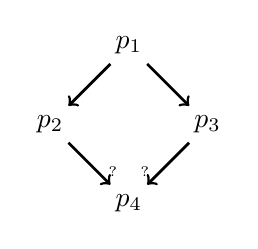
\begin{tikzpicture}
  \tikzset{
    esstep/.style={->,line width=0.35mm},
  }
  \node (p1) at (1,2) {$p_1$};
  \node (p2) at (0,1) {$p_2$};
  \node (p3) at (2,1) {$p_3$};
  \node (p4) at (1,0) {$p_4$};
  \draw[esstep] (p1) edge (p2);
  \draw[esstep] (p1) edge (p3);
  \draw[esstep] (p2) edge node[pos=0.7,right] {{\tiny?}} (p4);
  \draw[esstep] (p3) edge node[pos=0.7,left ] {{\tiny?}} (p4);
\end{tikzpicture}
\end{center}
%
\end{theorem}

\begin{lemma}
\label{lm:es-opsem-lang-mon}
Язык, задаваемый структурой событий, 
монотонно растёт при построении структуры 
с помощью системы переходов $\esStep{}$.
$$ p \esStep{} p' \implies \pomlang{S(p)} \suq \pomlang{S(p')} $$
\end{lemma}

\begin{theorem}[Полнота]
\label{thm:es-opsem-completeness}
Рассмотрим программу $P$ и модель памяти $M$,
такую что её язык $\wmmlang{M}$ префикс-замкнут.
Пусть $p$ это терминальный помсет, построенный с помощью операционной семантики, 
то есть $p_0(P) \esStep{}^* p$ и не существует $p'$ такого, что $p \esStep{} p'$.
Тогда структура событий событий $S(p)$ полна относительно
аксиоматической семантики программы $P$ в модели $M$:
$$ \sem{P}_M \suq \ExecGs{\wmmpes{S}{M}}. $$
\end{theorem}

\begin{proof}

Рассмотрим $G \in \sem{P}_M$ и соответствующий ему помсет ${q = \pomg[G]}$. 
Согласно \cref{lm:es-opsem-prefix-clos} можно заключить, что $p_0(P) \esStep{}^* q$.
Также, нетрудно убедиться, что $q \in \pomlang{S(q)}$.
Далee, использую свойство конфлюэнтности (\cref{thm:es-opsem-confluence}),
можно заключить, что существует $p'$, такой что 
$q \esStep{}^* p'$ и $p \esStep{}^* p'$.
По \cref{lm:es-opsem-lang-mon} имеем, что 
${q \in \pomlang{S(q)} \suq \pomlang{S(p')}}$.
Осталось лишь заметить, что так как $p$ терминальный помсет, то $p = p'$.

\begin{center}
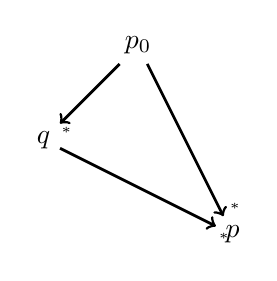
\begin{tikzpicture}[scale=1.2]
  \tikzset{
    esstep/.style={->,line width=0.35mm},
  }
  \node (p0) at (1,2) {$p_0$};
  \node (q)  at (0,1) {$q$};
  \node (p)  at (2,0) {$p$};
  \draw[esstep] (p0) edge node[pos=1.15,right] {{\tiny *}} (q);
  \draw[esstep] (p0) edge node[pos= .95,right] {{\tiny *}} (p);
  \draw[esstep] (q)  edge node[pos=1.15,left ] {{\tiny *}} (p);
\end{tikzpicture}
\end{center}

\end{proof}

